\chapter{SYSTEMATIC REVIEW METHODOLOGY 
\label{appendix:systematic_review}}

A systematic review following a rigorous and well-structured approach to summarizing and synthesizing the existing research was performed according to the methodology below. The first step was a search considering the following parameters:

\begin{itemize}
   \item \textbf{Search query}:  \enquote{sound AND recognition AND embedded}, \enquote{sound AND classification AND embedded}, \enquote{audio AND scene AND classification}, \enquote{audio AND scene AND recognition}, \enquote{auditory AND scene AND classification}, and \enquote{auditory AND scene AND recognition};
   \item \textbf{Knowledge databases}: \textit{sciencedirect.com}, \textit{scopus.com}, \textit{webofscience.com}, \textit{ieeexplore.ieee.org}, and \textit{semanticscholar.org};
   \item \textbf{Exclusion criterion}: none.
\end{itemize}
In total, 2.629 documents were selected from the search query:
\begin{itemize}
    \item{384 papers at IEEE Xplore};
    \item{341 papers at Semantics Scholar};
    \item{450 papers at Web of Science};
    \item{863 papers at ScienceDirect};
    \item{591 papers at Scopus}.
\end{itemize}

To start the screening and selection process, the bibliographic information of these documents was processed using a specialized software named VOSviewer for the purpose of establishing relationships through bibliographic coupling, co-citation, co-authorship, and co-occurrence of keywords, thus creating a dynamic and interactive bibliometric network with multiple layers (Figure \ref{fig:systematic_review_methodology_bibliometric_networks}) that allowed to analyze the strength between the nodes connecting each other as well the relationship between the keywords, authors, and co-authors. At the end of this process, 143 documents were selected.

For each identified document, a corresponding entry was registered in the software Zotero, enabling the analysis of the subsequent metrics:
 \begin{itemize}
   \item Number of explicit citations;
   \item Number of supportive citations;
   \item Number of contrasting citations.
 \end{itemize}

When the metrics were favorable, and the main objective of the selected document was related to the main objective of this study, the data extraction process began using the software Obsidian (Figure \ref{fig:systematic_review_methodology_obsidian}) to save the following information in a comprehensive report for the systematic review, adhering to the preferred reporting guidelines established in \gls{prisma}:
\begin{itemize}
    \item Document metadata;
    \item Keywords, citations, and references;
    \item The need for the research;
    \item The presented methodology;
    \item The final result and future works;
    \item Personal comments and remarks.
\end{itemize}

\begin{figure}[htbp]
    \raggedright
        \caption{Visualization of bibliometric networks.}
        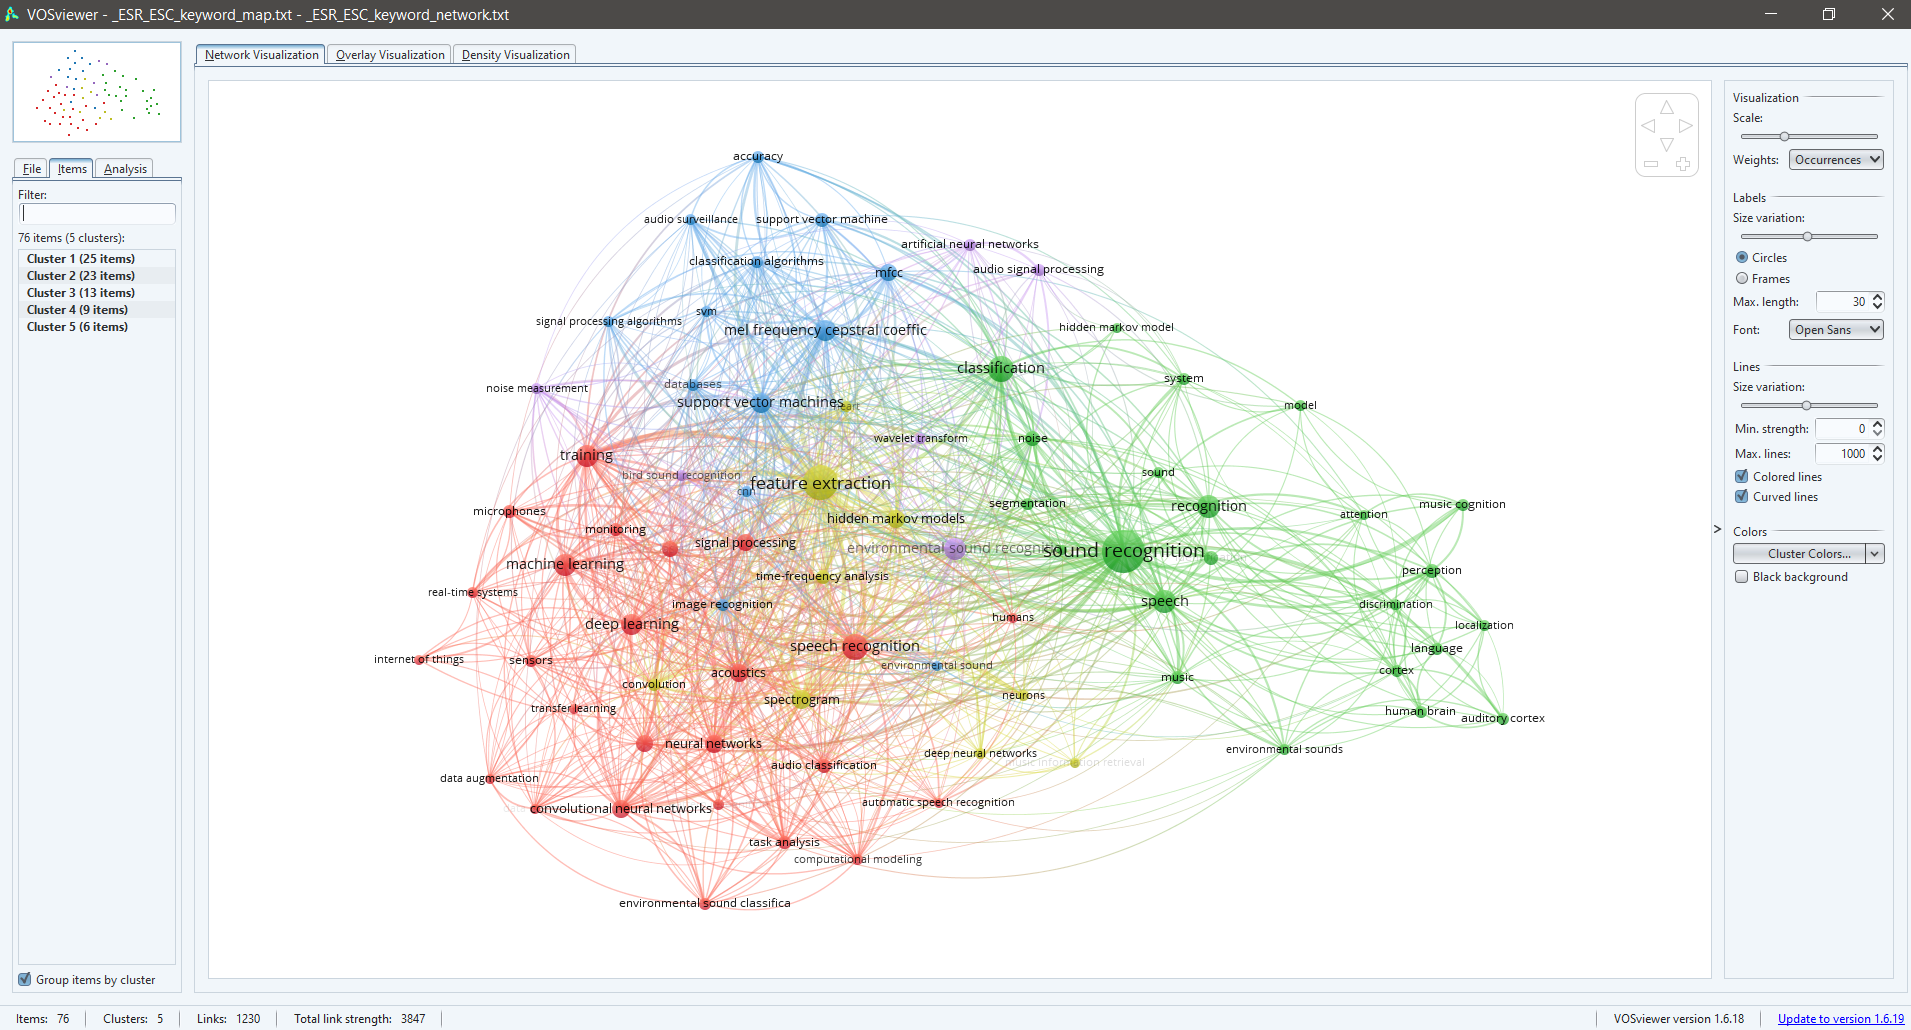
\includegraphics[width=0.80\textwidth]{resources/images/080-systematic_review/Review_VOSviewer_03_2023_01.png}
        \smallcaption{Source: Author}
        \label{fig:systematic_review_methodology_bibliometric_networks}
\end{figure}

\begin{figure}[htbp]
    \raggedright
        \caption{File structure in Obsidian for document data extraction.}
        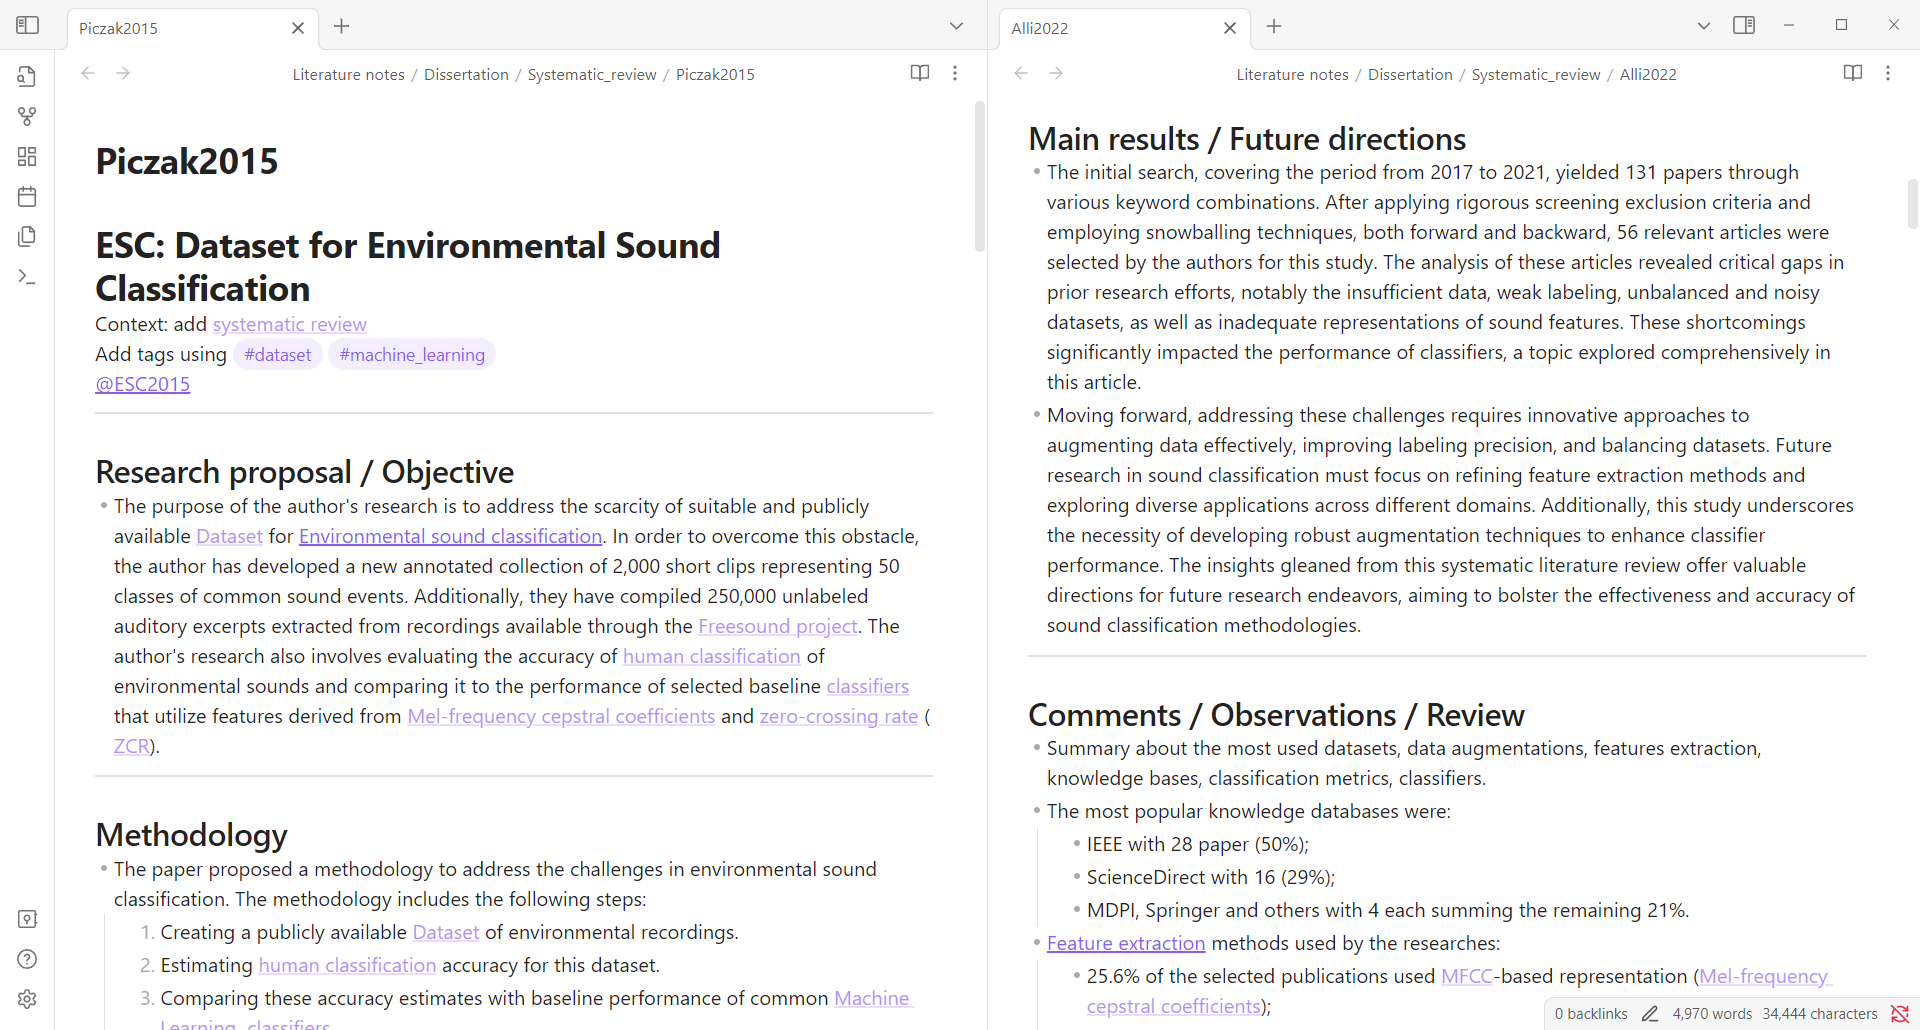
\includegraphics[width=0.80\textwidth]{resources/images/080-systematic_review/Review_Obsidian_01_2023_11.png}
        \smallcaption{Source: Author}
        \label{fig:systematic_review_methodology_obsidian}
\end{figure}

At the end of this stage, the Obsidian database contained 64 documents. After analyzing the information, 43 papers were selected as relevant. A detailed study of these documents was conducted, and the snowballing process was employed to identify additional relevant documents to complement the references.

Furthermore, references commonly used in the field of acoustics, machine learning, and neural networks, particularly those with a high number of citations, were not included in the aforementioned process.